%%%%%%%%%%%%%%%%%%%%%%%%%%%%%%%%%%%%%%%%%
% Beamer Presentation
% LaTeX Template
% Version 1.0 (10/11/12)
%
% This template has been downloaded from:
% http://www.LaTeXTemplates.com
%
% License:
% CC BY-NC-SA 3.0 (http://creativecommons.org/licenses/by-nc-sa/3.0/)
%
%%%%%%%%%%%%%%%%%%%%%%%%%%%%%%%%%%%%%%%%%

%----------------------------------------------------------------------------------------
%	PACKAGES AND THEMES
%----------------------------------------------------------------------------------------

\documentclass[]{beamer}

\mode<presentation> {
	
	% The Beamer class comes with a number of default slide themes
	% which change the colors and layouts of slides. Below this is a list
	% of all the themes, uncomment each in turn to see what they look like.
	
	%\usetheme{default}
	%\usetheme{AnnArbor}
	%\usetheme{Antibes}
	%\usetheme{Bergen}
	%\usetheme{Berkeley}
	%\usetheme{Berlin}
	%\usetheme{Boadilla}
	%\usetheme{CambridgeUS}
	%\usetheme{Copenhagen}
	%\usetheme{Darmstadt}
	%\usetheme{Dresden}
	%\usetheme{Frankfurt}
	%\usetheme{Goettingen}
	%\usetheme{Hannover}
	%\usetheme{Ilmenau}
	%\usetheme{JuanLesPins}
	%\usetheme{Luebeck}
	\usetheme{Madrid}
	%\usetheme{Malmoe}
	%\usetheme{Marburg}
	%\usetheme{Montpellier}
	%\usetheme{PaloAlto}
	%\usetheme{Pittsburgh}
	%\usetheme{Rochester}
	%\usetheme{Singapore}
	%\usetheme{Szeged}
	%\usetheme{Warsaw}
	
	% As well as themes, the Beamer class has a number of color themes
	% for any slide theme. Uncomment each of these in turn to see how it
	% changes the colors of your current slide theme.
	
	%\usecolortheme{albatross}
	%\usecolortheme{beaver}
	%\usecolortheme{beetle}
	%\usecolortheme{crane}
	%\usecolortheme{dolphin}
	%\usecolortheme{dove}
	%\usecolortheme{fly}
	%\usecolortheme{lily}
	%\usecolortheme{orchid}
	%\usecolortheme{rose}
	%\usecolortheme{seagull}
	%\usecolortheme{seahorse}
	%\usecolortheme{whale}
	%\usecolortheme{wolverine}
	
	%\setbeamertemplate{footline} % To remove the footer line in all slides uncomment this line
	%\setbeamertemplate{footline}[page number] % To replace the footer line in all slides with a simple slide count uncomment this line
	
	\setbeamertemplate{navigation symbols}{} % To remove the navigation symbols from the bottom of all slides uncomment this line
}

\makeatletter
\setbeamertemplate{footline}
{
	\leavevmode%
	\hbox{%
		\begin{beamercolorbox}[wd=.333333\paperwidth,ht=2.25ex,dp=1ex,center]{author in head/foot}%
			\usebeamerfont{author in head/foot}\insertsection
		\end{beamercolorbox}%
		\begin{beamercolorbox}[wd=.333333\paperwidth,ht=2.25ex,dp=1ex,center]{title in head/foot}%
			\usebeamerfont{title in head/foot}\insertsubsection
		\end{beamercolorbox}%
		\begin{beamercolorbox}[wd=.333333\paperwidth,ht=2.25ex,dp=1ex,right]{date in head/foot}%
			\usebeamerfont{date in head/foot}\insertshortdate{}\hspace*{2em}
			\insertframenumber{} / \inserttotalframenumber\hspace*{2ex} 
	\end{beamercolorbox}}%
	\vskip0pt%
}
\makeatother

\usepackage{graphicx} % Allows including images
\usepackage{booktabs} % Allows the use of \toprule, \midrule and \bottomrule in tables
\usepackage{amssymb,amsmath,dsfont,physics}
\usepackage[english]{babel}
\usefonttheme[onlymath]{serif}
\usepackage{multicol}
\usepackage{datetime,xcolor}
\usepackage{ragged2e} % for \justifying

\apptocmd{\frame}{}{\justifying}{}

% Definitions
\newcommand{\C}[1]{\ensuremath{\mathbb{C}^{#1}}}
\newcommand{\R}[1]{\ensuremath{\mathbb{R}^{#1}}}
\newcommand{\Exp}[2][]{\ensuremath{E_{#1}\qty[#2]}}
\newcommand{\Cov}[1]{\ensuremath{\text{Cov}\qty(#1)}}
\newcommand{\myspace}{\vspace{3mm}}
\newcommand{\herm}[1]{\ensuremath{#1^\dagger}}
\newcommand{\vt}[1]{\ensuremath{\tilde{\vb{#1}}}}
\newcommand{\cscg}{circularly symmetric Complex Gaussian}

% Custom colors
\definecolor{DEIred}{RGB}{153,14,32}
\definecolor{darkDEI1}{RGB}{117,11,24}
\definecolor{darkDEI2}{RGB}{78,7,16}
\definecolor{darkDEI3}{RGB}{117,11,24}

\setbeamercolor{palette primary}{bg=DEIred,fg=white}
\setbeamercolor{palette secondary}{bg=darkDEI1,fg=white}
\setbeamercolor{palette tertiary}{bg=darkDEI2,fg=white}
\setbeamercolor{palette quaternary}{bg=darkDEI3,fg=white}
\setbeamercolor{structure}{fg=DEIred} % itemize, enumerate, etc
\setbeamercolor{section in toc}{fg=black} % TOC sections
% Override palette coloring with secondary
\setbeamercolor{subsection in head/foot}{bg=blue,fg=white}

%----------------------------------------------------------------------------------------
%	TITLE PAGE
%----------------------------------------------------------------------------------------

\title[Notation]{Capacity of Multi-antenna Gaussian Channels\\
	(I. E. Telatar, 1999)} % The short title appears at the bottom of every slide, the full title is only on the title page

\author[Lecci]{Mattia Lecci\inst{1}\inst{2}} % Your name

\institute[UniPD/UPC] % Your institution as it will appear on the bottom of every slide, may be shorthand to save space
{
	\inst{1}
	Universit\`a degli Studi di Padova\\
	Department of Information Engineering\\
	(DEI-UniPD)
	\and
	\inst{2}
	Universitat Polit\`{e}cnica de Catalunya\\ % Your institution for the title page
	Escola T\`ecnica Superior d'Engenyeria de Telecomunicaci\'o  de Barcelona\\
	(UPC-ETSETB)
	%\medskip
	%\textit{javier.fonollosa@upc.edu} % Your email address
}
\date{January 2018} % Date, can be changed to a custom date


%------------------------------------------------------------
%------------------------------------------------------------
%The next block of commands puts the table of contents at the 
%beginning of each section and highlights the current section:

\AtBeginSection[]
{
	\begin{frame}
	\frametitle{Table of Contents}
	\tableofcontents[currentsection]
\end{frame}
}
%------------------------------------------------------------


\begin{document}
\begin{frame}
\titlepage % Print the title page as the first slide
\begin{figure}
	\hspace{2cm}
	
\includegraphics[height = 1.2cm]{img/dei_logo}
	\hfill
	
\includegraphics[height = 1.2cm]{img/ETSETB-positiu-p3005}
	\hspace{1cm}
\end{figure}
\end{frame}

\begin{frame}
\frametitle{Overview} % Table of contents slide, comment this block out to remove it
%\begin{multicols}{2}
	\tableofcontents
%\end{multicols}
\end{frame}

\section{Introduction}

\subsection{Abstract}
%%%%%%%%%%%%%%%%%%%%%%%%%%%%%%%%%%%%%%%%%%%%%%%%%%%%%%%%%
\begin{frame}{Abstract}
In this presentation I will talk about the capacity of a single-user Gaussian channel with multiple receiving and/or transmitting antennas \cite{telatar99} (also known as \alert{MIMO} channel).

\myspace
I will talk about 3 cases:
\begin{itemize}
	\item Deterministic channel
	\item Random i.i.d. ergodic channel
	\item \textit{Bonus}: multi-user case
\end{itemize}

\end{frame}

%%%%%%%%%%%%%%%%%%%%%%%%%%%%%%%%%%%%%%%%%%%%%%%%%%%%%%%%%%
\subsection{Notation and Assumptions}
\begin{frame}[allowframebreaks]{Notation}
The notation adopted is halfway between the one used during the course and the one from the original paper.

\myspace
Let's denote with $t$ the number of transmitting and with $r$ the number of receiving antennas.

\myspace
We will consider the classical linear model, where $\vb{x}\in \C{t}$ is the transmitted vector and $\vb{y}\in \C{r}$ is the received vector, $H\in \C{r\times t}$ is the complex channel matrix and $\vb{n}\in \C{r}$ is the noise
$$\vb{y} = H\vb{x} + \vb{n}$$

%%%%%%%%%%%%%%%%%%%%%%%%%%%%%%%%%%%%%%%%%%%%%%%%%%%%%%%%%%
\framebreak

We assume noise at different receivers to be independent and normalized, i.e. $\Exp{\vb{n} \herm{\vb{n}}} = I_r$.\\
The dag (\dag) notation is used for the conjugate-transpose operation.

\myspace
We have the power constraint
$$\Exp{\herm{\vb{x}}\vb{x}} = \Exp{\tr(\vb{x}\herm{\vb{x}})} = \tr(\Exp{\vb{x}\herm{\vb{x}}})\leq P$$

\myspace
A complex random vector (r.ve.) $\vb{x}\in \C{n}$ is said to be Complex Gaussian if its real extension $\vh{x} \triangleq \qty[\begin{array}{c}
\Re{\vb{x}}\\
\Im{\vb{x}}
\end{array}]
\in \R{2n}$ is Gaussian.

\myspace
The r.ve. $\vb{x}$ will have \textit{mean} and \textit{covariance} respectively $\mu= \Exp{\vb{x}}$ and $Q = \Cov{Q} = \Exp{(\vb{x}-\mu)\herm{(\vb{x}-\mu)}}$

%%%%%%%%%%%%%%%%%%%%%%%%%%%%%%%%%%%%%%%%%%%%%%%%%%%%%%%%%%
\framebreak

Defining for a complex matrix $A$
$$\hat{A} = \qty[\begin{array}{lr}
\Re(A) & -\Im(A)\\
\Im(A) & \Re(A)
\end{array}]$$
we say that a Complex Gaussian r.ve. is \textit{circularly symmetric} if
$$\Cov{\vh{x}} = \Exp{(\vh{x}-\hat{\mu})(\vh{x}-\hat{\mu})^T} = \frac{1}{2} \hat{Q}$$

\begin{block}{pdf of \cscg}
	The pdf of a \cscg is
	\begin{align*}
	\begin{split}
	\gamma_{\mu,Q} &= \det(\pi\hat{Q})^{-\frac{1}{2}} e^{-(\hat{x}-\hat{\mu})^T\hat{Q}(\hat{x}-\hat{\mu})}\\
	&= \det(\pi Q)^{-1} e^{-\herm{(x-\mu)}Q(x-\mu)}
	\end{split}
	\end{align*}
\end{block}

\end{frame}

%%%%%%%%%%%%%%%%%%%%%%%%%%%%%%%%%%%%%%%%%%%%%%%%%%%%%%%%%%
\subsection{Properties and Lemmas}
\begin{frame}[allowframebreaks]{Properties and Lemmas}
\begin{block}{Lemma 1}
	The following properties hold:
	\begin{subequations}
	\begin{gather}
	C=AB \iff \hat{C} = \hat{A}\hat{B}\\
	C = A+B \iff \hat{C} = \hat{A} + \hat{B}\\
	C = \herm{A} \iff \hat{C}=\hat{A}^T\\
	C=A^{-1} \iff \hat{C} = \hat{A}^{-1}\\
	\det(\hat{A}) = |\det(A)|^2 = \det(A \herm{A})\\
	z = x+y \iff \hat{z} = \hat{x}+\hat{y}\\
	y=Ax \iff \hat{y} = \hat{A}\hat{x}\\
	\Re{\herm{x}y} = \hat{x}^T\hat{y}
	\end{gather}
	\end{subequations}
\end{block}

%%%%%%%%%%%%%%%%%%%%%%%%%%%%%%%%%%%%%%%%%%%%%%%%%%%%%%%%%%
\framebreak

\begin{block}{Corollary 1}
A matrix $U\in \C{n\times n}$ is unitary if and only if $\hat{U}\in \R{2n\times 2n}$ is orthonormal.
\end{block}
\begin{block}{Corollary 2}
If $Q\in \C{n\times n}$ is positive semi-definite, then so is $\hat{Q}\in \R{2n\times 2n}$.
\end{block}
\begin{alertblock}{Lemma 2}\justify
Suppose the complex r.ve. $\vb{x}\in \C{n}$ is
zero-mean and $\Cov{\vb{x}}=Q$.\\
Then the differential entropy of $\vb{x}$ satisfies $h(\vb{x}) \leq \log\det(\pi e Q)$ with equality if and only if $\vb{x}$ is \cscg.
\end{alertblock}
In other words, \cscg r.ve. are entropy maximizers for the class of complex random vectors.

%%%%%%%%%%%%%%%%%%%%%%%%%%%%%%%%%%%%%%%%%%%%%%%%%%%%%%%%%%
\framebreak

\begin{block}{Lemma 3}
lf $\vb{x}\in \C{n}$ is a \cscg then so is $\vb{y} = A\vb{x}$ for any $A \in \C{m\times n}$.
\end{block}
\begin{block}{Lemma 4}\label{lemma:4}
	f $\vb{x}$ and $\vb{y}$ are independent {\cscg s}, then $\vb{z}=\vb{x}+\vb{y}$ is also \cscg.
\end{block}

\end{frame}

%%%%%%%%%%%%%%%%%%%%%%%%%%%%%%%%%%%%%%%%%%%%%%%%%%%%%%%%%%
%%%%%%%%%%%%%%%%%%%%%%%%%%%%%%%%%%%%%%%%%%%%%%%%%%%%%%%%%%
\section{Gaussian Channel with Deterministic $H$}
%%%%%%%%%%%%%%%%%%%%%%%%%%%%%%%%%%%%%%%%%%%%%%%%%%%%%%%%%%%%%%%%%%%
%%%%%%%%%%%%%%%%%%%%%%%%%%%%%%%%%%%%%%%%%%%%%%%%%%%%%%%%%%%%%%%%%%%
\subsection{Capacity Derivation}
\begin{frame}[allowframebreaks]{Capacity Derivation}
We first consider the case of a deterministic (fixed) transfer function $H$. Note that the capacity is a function of both the transfer function and the power constraint, i.e. $C(H,P)$. We consider the case where both receiver and transmitter know the matrix $H$.

\begin{block}{Singular Value Decomposition (SVD)}\justify
Any matrix $H\in \C{r\times t}$ can be decomposed as
$$H = UD\herm{V}$$
where $U\in \C{r\times r}$ and $V \in \C{t\times t}$ are unitary, $D\in \C{r\times t}$ is diagonal with non-negative real entries.

In fact, the columns of $U$ are the eigenvectors of $H\herm{H}$, the columns of $V$ are the eigenvectors of $\herm{H}H$ and the diagonal entries of $D$, called \textit{singular values} of $H$, are the eigenvalues, which coincide for the two cases and given the hermitianity of such matrices, they are real and non-negative.
\end{block}

%%%%%%%%%%%%%%%%%%%%%%%%%%%%%%%%%%%%%%%%%%%%%%%%%%%%%%%%%%%%%%%%%%%
\framebreak

Thus, the problem can be seen as follows
$$\vb{y} = UD\herm{V}\vb{x} + \vb{n}$$

Therefore, preprocessing the transmitted symbol as $\vb{x} = V\vt{x}$ and $\vt{y}=\herm{U}\vb{y}$ and defining $\vt{n} = \herm{U}\vb{n}$, we get
$$\vt{y} = D\vt{x} + \vt{n}$$
as an equivalent channel.

\myspace
Calling $\sigma_i = \lambda_i^{\frac{1}{2}}$ the singular values for $i=1,\ldots,\min(r,t)$, we have
\begin{equation*}
\begin{cases}
\tilde{\vb{y}}_i = \sigma_i \tilde{\vb{x}}_i + \tilde{\vb{n}}_i & 1\leq i\leq \min(r,t)\\
\tilde{\vb{y}}_i = \tilde{\vb{n}}_i & i > \min(r,t)
\end{cases}
\end{equation*}

%%%%%%%%%%%%%%%%%%%%%%%%%%%%%%%%%%%%%%%%%%%%%%%%%%%%%%%%%%%%%%%%%%%
\framebreak

It's clear that in order to maximize the capacity we need to choose $\vt{\vb{x}}_i$ for $1\leq i \leq \min(r,t)$ (actually only up to the number of non-zero singular values) to be independent, zero-mean, \cscg.

\medskip
It can be shown that the optimal variances must follow once again the "water-filling" equations
\begin{equation*}
\begin{cases}
\Exp{\Re(\vt{\vb{x}}_i)} = \Exp{\Im(\vt{\vb{x}}_i)} = \frac{1}{2} \qty(\mu-\lambda_i^{-1})^+\\
P = \sum_i \qty(\mu-\lambda_i^{-1})^+\\
C = \sum_i \qty(\log(\mu\lambda_i))^+
\end{cases}
\end{equation*}

\end{frame}

%%%%%%%%%%%%%%%%%%%%%%%%%%%%%%%%%%%%%%%%%%%%%%%%%%%%%%%%%%%%%%%%%%%
%%%%%%%%%%%%%%%%%%%%%%%%%%%%%%%%%%%%%%%%%%%%%%%%%%%%%%%%%%%%%%%%%%%
\subsection{Examples}
\begin{frame}
\begin{example}{Example 1}
	MAYBE??????
\end{example}
\end{frame}

%%%%%%%%%%%%%%%%%%%%%%%%%%%%%%%%%%%%%%%%%%%%%%%%%%%%%%%%%%%%%%%%%%%
%%%%%%%%%%%%%%%%%%%%%%%%%%%%%%%%%%%%%%%%%%%%%%%%%%%%%%%%%%%%%%%%%%%
\subsection{Formal Derivation of Capacity}
\begin{frame}[allowframebreaks]{Formal Derivation of Capacity}

I will now proceed in the derivation of the capacity in a more formal way. This also will be used with some slight differences in the derivation of the capacity when $\vb{H}$ is not deterministic.

\medskip
Recall, the mutual information that we are interested in is
$$I(\vb{x};\vb{y}) = h(\vb{y})-h(\vb{y}|\vb{x}) = h(\vb{y})-h(\vb{n})$$

Note that if $\vb{x}$ satisfies $\Exp{\herm{\vb{x}}\vb{x}} \leq P$, so does $\vb{x}-\Exp{\vb{x}}$, thus we will only focus on zero-mean $\vb{x}$.

\medskip
Furthermore, if $\vb{x}$ is zero-mean with covariance $\Exp{\vb{x}\herm{\vb{x}}} = Q$, then $\vb{y}$ is zero-mean with covariance $\Exp{\vb{y}\herm{\vb{y}}} = HQ\herm{H} + I_r$, and by Lemma 2 among such $\vb{y}$ the entropy is largest when $\vb{y}$ is \cscg, which is the case when $\vb{x}$ is \cscg{} (Lemmas 3 and 4).

%%%%%%%%%%%%%%%%%%%%%%%%%%%%%%%%%%%%%%%%%%%%%%%%%%%%%%%%%%%%%%%%%%%
\framebreak

Considering, then, $\vb{x}$ \cscg, we have
\begin{align*}
\begin{split}
I(\vb{x;y}) &= h(\vb{y})-h(\vb{n}) = \log\det(\pi e(I_r + HQ\herm{H})) - \log\det(\pi e I_r)\\
&= \log\det(I_r + HQ\herm{H}) = \log\det(I_t + Q\herm{H}H)
\end{split}
\end{align*}
where the last equality is given by \textit{Sylvester's determinant identity}, that states $\det(I+AB) = \det(I+BA)$.

\medskip
Since it occurs many times during the paper, we define
$$\Psi(Q,H) = \log\det(I_r + HQ\herm{H})$$

%%%%%%%%%%%%%%%%%%%%%%%%%%%%%%%%%%%%%%%%%%%%%%%%%%%%%%%%%%%%%%%%%%%
\framebreak

Since we're dealing with zero-mean \cscg, we only need to find a positive semi-definite matrix $Q$ to fully determine the distribution, such that $\tr(Q)\leq P$.

\medskip
Notice that $\herm{H}H$ is hermitian, thus it can be decomposed as $\herm{H}H = \herm{V}\Lambda V$ with unitary $V$ and diagonal positive semi-definite $\Lambda$. Thus, using Sylvester's identity again we obtain
\begin{align*}
\begin{split}
\log\det(I_t + Q\herm{H}H) &=
\log\det(I_t + \Lambda^\frac{1}{2}VQ\herm{V}\Lambda^\frac{1}{2})\\
&= \log\det(I_t + \Lambda^\frac{1}{2}\tilde{Q}\Lambda^\frac{1}{2})
\end{split}
\end{align*}
where we noticed that $Q$ and $\tilde{Q}$ are equivalent for both definiteness and power constraint, so we can as well optimize over $\tilde{Q}$.

%%%%%%%%%%%%%%%%%%%%%%%%%%%%%%%%%%%%%%%%%%%%%%%%%%%%%%%%%%%%%%%%%%%
\framebreak

A special case of \textit{Hadamard's inequality} for positive semi-definite matrices, states that
$$I(\vb{x;y})
= \log\det(I_t + \Lambda^\frac{1}{2}\tilde{Q}\Lambda^\frac{1}{2})
\leq \prod_i (1+ \tilde{Q}_{ii}\lambda_i) $$
with equality for diagonal matrices.

Thus, we see that the maximizing $\tilde{Q} = VQ\herm{V}$ is diagonal, and the optimal entries follow the water-filling equations, i.e.
\begin{equation*}
\begin{cases}
\tilde{Q}_{ii} = (\mu-\lambda_i^{-1})^+\\
P = \sum_i \tilde{Q}_{ii}\\
C = \sum_i (\log(\mu\lambda_i))^+
\end{cases}
\end{equation*}

\end{frame}
\section{Gaussian Channel with Ergodic $\vb{H}$}
%%%%%%%%%%%%%%%%%%%%%%%%%%%%%%%%%%%%%%%%%%%%%%%%%%%%%%%%%%%%%%%%%%%
%%%%%%%%%%%%%%%%%%%%%%%%%%%%%%%%%%%%%%%%%%%%%%%%%%%%%%%%%%%%%%%%%%%
\subsection{Introduction to the problem}
\begin{frame}{Introduction}

We now consider the case when the matrix $\vb{H}$ is i.i.d. random and ergodic. Ergodicity comes into play to ensure that the capacity is the actual bound as as matrix is randomly changing over time.

\medskip
We assume that $\vb{H}$ is independent of both $\vb{x}$ and $\vb{n}$, and that the specific realization $H$ is know at the receiver (while the transmitter only knows it's distribution). Thus, we can equivalently say that the channel yields the couple $(\vb{y,H})$.

\medskip
We will further assume that the entry of $\vb{H}$ are i.i.d. zero-mean Complex Gaussians, with independent real and imaginary parts, each with variance $\frac{1}{2}$.

\medskip
In other words we are considering a Rayleigh fading channel for each component and enough physical separation within transmitting and receiving antennas to achieve independence between the entries of $\vb{H}$.

\end{frame}

%%%%%%%%%%%%%%%%%%%%%%%%%%%%%%%%%%%%%%%%%%%%%%%%%%%%%%%%%%%%%%%%%%%
%%%%%%%%%%%%%%%%%%%%%%%%%%%%%%%%%%%%%%%%%%%%%%%%%%%%%%%%%%%%%%%%%%%
\subsection{Capacity-achieving Distribution}
\begin{frame}[allowframebreaks]{Capacity-achieving Distribution}
This time, we can compute the mutual information as follows
\begin{align*}
\begin{split}
I(\vb{x;(y,H)}) &= I(\vb{x;H}) + I(\vb{x;y|H})\\
&= I(\vb{x;y|H})\\
&= \Exp[\vb{H}]{I(\vb{x;y|H}=H)}
\end{split}
\end{align*}

We know that for a deterministic $H$, the maximizer $\vb{x}$ takes the form of a zero-mean \cscg{} with covariance $Q$, and $\Psi(Q,H) = \log\det(I_r + HQ\herm{H})$ is the corresponding maximal mutual information.

\medskip
We thus need to maximize
$$\Psi(Q) = \Exp{\Psi(Q,\vb{H})} = \Exp{\log\det(I_r + \vb{H}Q\herm{\vb{H}})}$$
over the choice of positive semi-definite $Q$, such that $\tr(Q)\leq P$.

%%%%%%%%%%%%%%%%%%%%%%%%%%%%%%%%%%%%%%%%%%%%%%%%%%%%%%%%%%%%%%%%%%%
\framebreak

Since Q is positive semi-definite, we can write it as $Q = W\Delta\herm{W}$, where $W$ is unitary and $\Delta$ is non-negative diagonal. Thus
$$\Psi(Q) = \Exp{\log\det(I_r + (\vb{H}W)\Delta\herm{(\vb{H}W)})}$$
It can be shown that $\vb{H}W$ has the same distribution as $\vb{H}$ (since $W$ is unitary and $\vb{H}$ has i.i.d. entries), and thus $\Psi(Q)=\Psi(\Delta)$. It follows that we can focus on non-negative diagonal $Q$.

\medskip
Consider the permutation matrix $\Pi$ (which is orthogonal, thus unitary) and define $Q^\Pi \triangleq \Pi Q \Pi^T$. Again, we note that $\Psi(Q^\Pi) = \Psi(Q)$. Also, note that if $Q$ is diagonal, also $Q^\Pi$ is diagonal and they share the same determinant (the main diagonal is only shuffled).

%%%%%%%%%%%%%%%%%%%%%%%%%%%%%%%%%%%%%%%%%%%%%%%%%%%%%%%%%%%%%%%%%%%
\framebreak

Note that the transformation $Q\rightarrow I_r+HQ\herm{H}$ is linear and preserves positive definiteness, and know that the $\log\det$ function is concave over the closed cone of positive semi-definite matrices.\\
Thus $Q\rightarrow \Psi(Q)$ is concave.

\medskip
Let's define
$$\tilde{Q} = \frac{1}{t!}\sum_\Pi Q^\Pi$$
Note that $\tilde{Q}=\alpha I$ for some $\alpha$ for any $Q$, that $\tr(\tilde{Q})=\tr(Q)$ and $\Psi(\tilde{Q})\geq\Psi(Q)$.
%\begin{align*}
%\begin{split}
%\Psi(\tilde{Q}) &= \Psi\qty(\sum_\Pi \frac{1}{t!} Q^\Pi)
%\geq \sum_\Pi \frac{1}{t!} \Psi(Q^\Pi)
%\end{split}
%\end{align*}

%%%%%%%%%%%%%%%%%%%%%%%%%%%%%%%%%%%%%%%%%%%%%%%%%%%%%%%%%%%%%%%%%%%
\framebreak

\begin{theorem}
	The capacity of the channel is achieved when $\vb{x}$ is a \cscg{} with zero-mean and covariance $Q=\frac{P}{t}I_t$.\\
	The capacity is given by
	$$\Exp{\log\det(I_r + \frac{P}{t}\vb{H\herm{H}})}$$.
\end{theorem}

Note that for fixed $r$, by the Law of Large Numbers $\frac{1}{t}\vb{H\herm{H}} = I_r$, almost surely as $t$ gets large.\\ Thus, the capacity in the limit of large $t$ equals
$$r\log(1+P)$$
which scales linearly with the number of receivers!

\end{frame}

%%%%%%%%%%%%%%%%%%%%%%%%%%%%%%%%%%%%%%%%%%%%%%%%%%%%%%%%%%%%%%%%%%%
%%%%%%%%%%%%%%%%%%%%%%%%%%%%%%%%%%%%%%%%%%%%%%%%%%%%%%%%%%%%%%%%%%%
\subsection{Evaluation of the Capacity}
\begin{frame}[allowframebreaks]{Evaluation of the Capacity}

First of all, from the Sylvester's determinant identity we know that
$$\det(I_r + \frac{P}{t}\vb{H\herm{H}}) = \det(I_t + \frac{P}{t}\vb{\herm{H}H})$$
We can then define
\begin{equation*}
\vb{W}=\begin{cases}
\vb{H\herm{H}}	& r<t\\
\vb{\herm{H}H}	& r\geq t
\end{cases}
\end{equation*}
and also $m=\min(r,t)$, $M=\max(r,t)$.

\medskip
Clearly, $\vb{W}\in \C{m\times m}$ is a random positive semi-definite matrix, thus it has random, real, non-negative eigenvalues $\vb*{\lambda}_1,\ldots,\vb*{\lambda}_m$.

%%%%%%%%%%%%%%%%%%%%%%%%%%%%%%%%%%%%%%%%%%%%%%%%%%%%%%%%%%%%%%%%%%%
\framebreak

From the literature, we know that the entries of $\vb{W}$ follow a \textit{Wishart distribution with parameters $m$, $M$} and the joint density of the \textit{ordered} eigenvalues is known to be \cite{james1964}
$$p_{\lambda,\text{ord}} = 	\frac{1}{K_{m,M}}
\prod_i e^{-\lambda_i}\lambda_i^{M-m}
\prod_{j>i} (\lambda_i-\lambda_j)^2,
\quad \lambda_1\geq \ldots \geq \lambda_m \geq 0 $$
where $K_{m,M}$ is a normalizing factor.

\medskip
After many complex calculations and transformations we reach...

%%%%%%%%%%%%%%%%%%%%%%%%%%%%%%%%%%%%%%%%%%%%%%%%%%%%%%%%%%%%%%%%%%%
\framebreak

\begin{theorem}
	The capacity of the Gaussian Channel with ergodic matrix $\vb{H}$, with $t$ transmitters and $r$ receivers under power constraint $P$ equals
	\begin{equation}\label{eq:capacity_ergodic}
	\int_0^\infty \log(1+\frac{P}{t}\lambda)
	\sum_{k=0}^{m-1} \frac{k!}{(k+M-m)!}
	L_k^{M-m}(\lambda)^2
	\lambda^{M-m} e^{-\lambda}
	\dd{\lambda}
	\end{equation}
	where $m=\min(r,t)$, $M=\max(r,t)$, and
	$$L_k^{M-m}(x) = \frac{1}{k!}
	e^x x^{m-M}
	\dv[k]{}{x}
	\qty(e^{-x}x^{M-m+k})$$
	are the \textit{associated Laguerre polynomials}.
\end{theorem}

\end{frame}

%%%%%%%%%%%%%%%%%%%%%%%%%%%%%%%%%%%%%%%%%%%%%%%%%%%%%%%%%%%%%%%%%%%
%%%%%%%%%%%%%%%%%%%%%%%%%%%%%%%%%%%%%%%%%%%%%%%%%%%%%%%%%%%%%%%%%%%
\subsection{Examples}
\begin{frame}[allowframebreaks]{Examples}

\begin{example}[$t=1$]
	In this case $m=1$ and $M=r$. Note that $L_0^{r-1}(\lambda)=1$, thus from Eq.~\eqref{eq:capacity_ergodic} we get
	$$C = \frac{1}{(r-1)!}
	\int_0^\infty \log(1+P\lambda)
	\lambda^{r-1} e^{-\lambda}
	\dd{\lambda}$$
	As $r$ gets large, so does the capacity.
	
	It can be shown that as $r\rightarrow\infty$, $C \sim \log(1+rP)$, meaning that $C-\log(1+rP) \xrightarrow{r\rightarrow\infty} 0$.
\end{example}

\begin{example}[$t=1$]
\begin{figure}
	\centering
	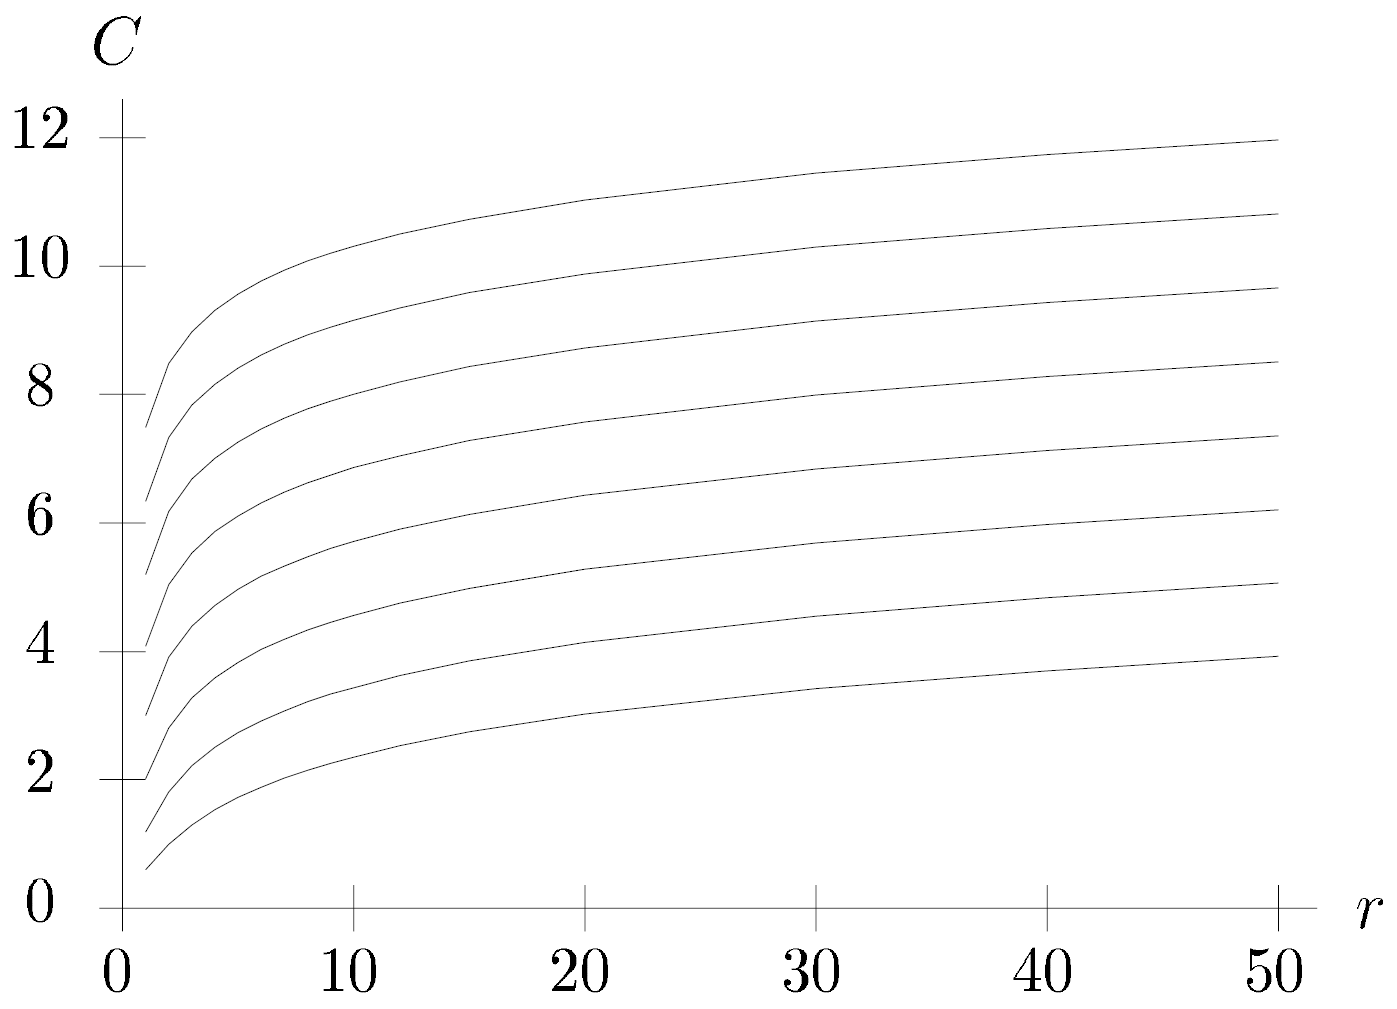
\includegraphics[width=0.6\linewidth]{img/capacity_t1}
	\caption{The value of the capacity (in \textit{nats}) for $0$dB$\leq P\leq 35$dB in $5$dB increments}
	\label{fig:capacity_t1}
\end{figure}
\end{example}

\begin{example}[$r=1$]
	In this case $m=1$ and $M=t$. Differently from before, though, the capacity is
	$$C = \frac{1}{(t-1)!}
	\int_0^\infty \log(1+\frac{P}{t}\lambda)
	\lambda^{t-1} e^{-\lambda}
	\dd{\lambda}$$
	Quite differently from before, the asymptotic capacity is $C \xrightarrow{t\rightarrow\infty} \log(1+P)$.
	
	Thus, just increasing the number of transmitting antennas will not help getting more capacity.
\end{example}

\begin{example}[$r=1$]
	\begin{figure}
		\centering
		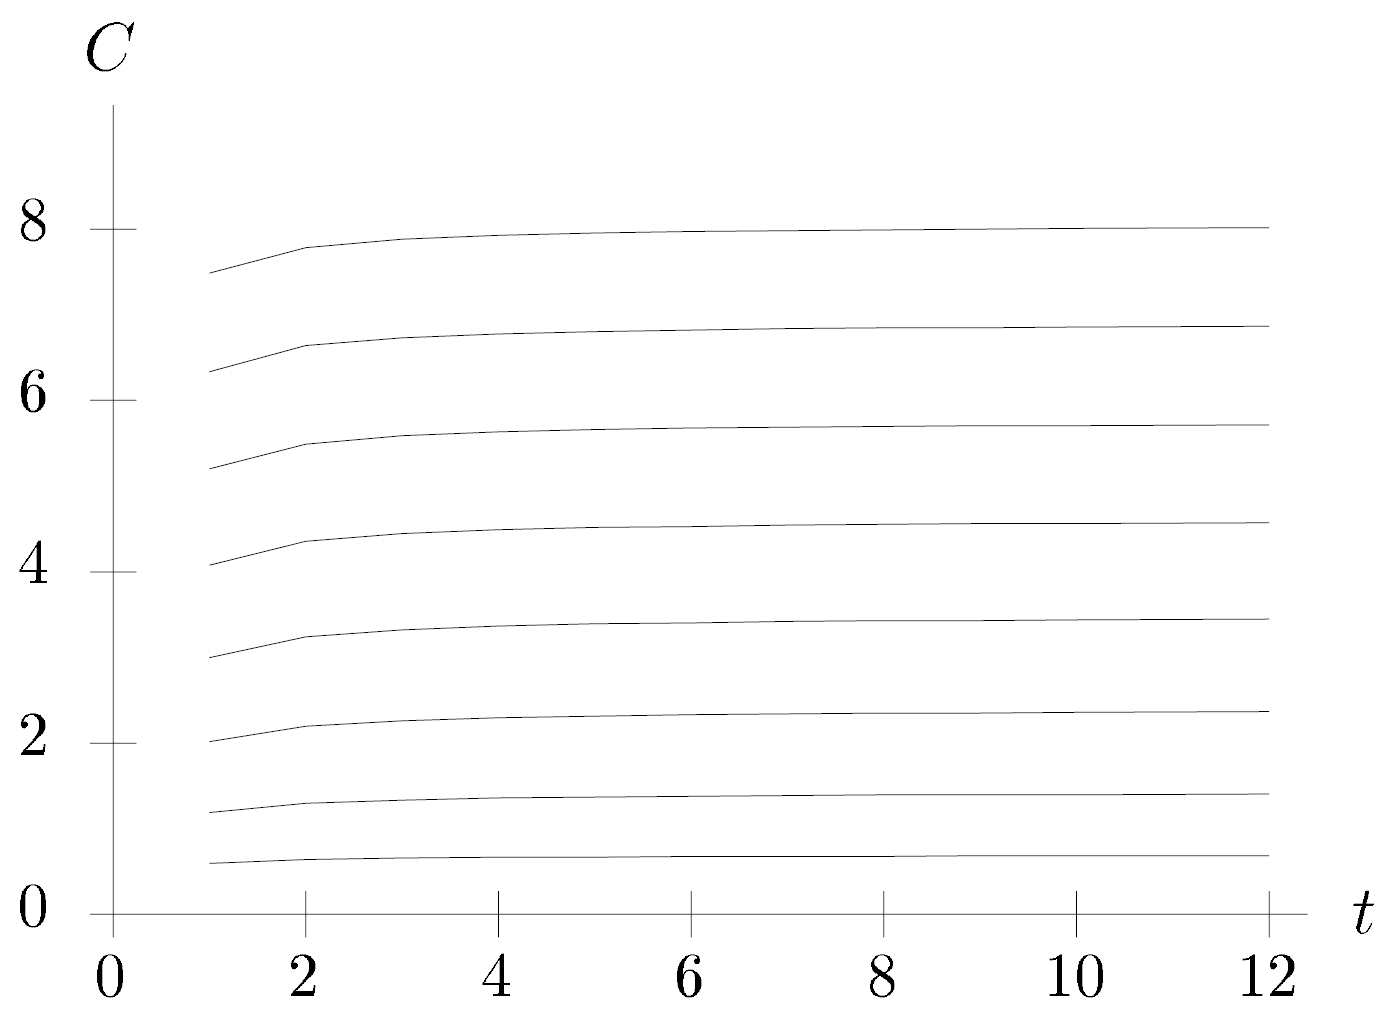
\includegraphics[width=0.6\linewidth]{img/capacity_r1}
		\caption{The value of the capacity (in \textit{nats}) for $0$dB$\leq P\leq 35$dB in $5$dB increments}
		\label{fig:capacity_r1}
	\end{figure}
\end{example}

\begin{example}[$r=t$]
	In this case $m=M=r=t$. From Eq.~\eqref{eq:capacity_ergodic}, then, we get
	$$C =
	\int_0^\infty \log(1+\frac{P}{m}\lambda)
	\sum_{k=0}^{m-1} L_k(\lambda)^2 e^{-\lambda}
	\dd{\lambda}$$
	There actually exists a close form formula for this integral, which is
	\begin{equation}
	\lim_{m\rightarrow\infty} \frac{C}{m} =
	\log P -1+ \frac{\sqrt{1+4P}-1}{2P} + 2\tanh[-1](\frac{1}{\sqrt{1+4P}})
	\end{equation}
	which clearly means that the capacity is a linear function of the number of transmitting/receiving antennas.
\end{example}

\begin{example}[$r=t$]
	\begin{figure}
		\centering
		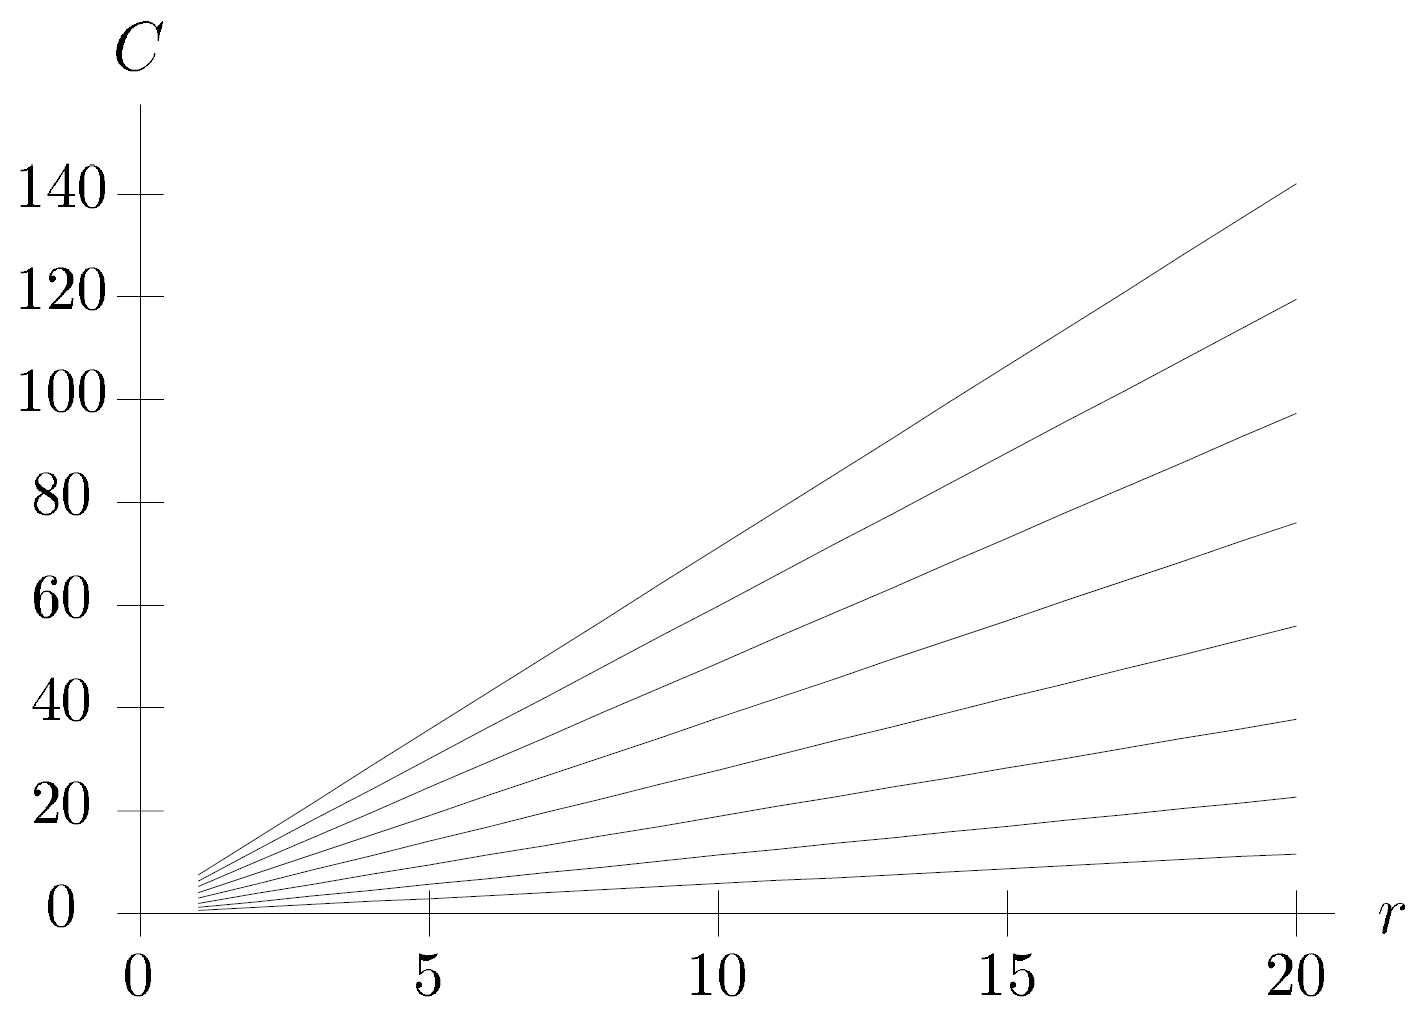
\includegraphics[width=0.7\linewidth]{img/capacity_rt}
		\caption{The value of the capacity (in \textit{nats}) for $0$dB$\leq P\leq 35$dB in $5$dB increments}
		\label{fig:capacity_rt}
	\end{figure}
\end{example}

\end{frame}

\begin{frame}{References}
\nocite{*}
\bibliographystyle{ieeetr}
\bibliography{mybib}
\end{frame}

\end{document} 